\documentclass[../TGMAFFIRO]{subfiles}

\begin{document}
% TODO: set context: why is it true that the value of something has been of great importance?

Throughout modern history, the value of \textit{anything} has been of great importance. For any two members taking opposite sides of a desired object\footnote{In other words, one member wants to buy (obtain) and the other member to sell (get rid off)}, an exchange takes place if they both agree on the current worth of the object to exchange. For this to happen, both members must be able to find one another. It may also be the case for either of the two to find a third whose worth of the object at play favors them more.\\

A \textbf{security} is the epitome of a tradable object in financial markets. We define a security as an instrument that either represents ownership or that derives its value from a commodity. We say that a security is \textbf{fungible} if any unit of the instrument is economically indistinguishable from all other units. That is, whoever buys (or sells) the instrument can pay (or receive) any unit at the same price at a given point in time.\\

The problem of searching for the price and the party whose view on the value of a security reflect ours is called \textbf{trading}. A \textbf{market} is the place where buyers meet sellers. Markets can be either a physical place (called a trading floor) or an electronic system\\

Not all financial products are traded in formal markets. Over the counter (OTC) trades happen between two parties directly or via a broker, who helps them settle the trade. 

\section{The Participants}
In a financial market, participants have various reasons to trade. On the one hand there is the \textbf{buy-side}. They trade in order to solve a financial problem originated outside of the market. This group sees the market as a means to an end, and thus, they rely on the resources available in the market.\\

\begin{table}[!h]
	\centering
	\begin{tabular}{ c c m{3cm} c}
		\hline
		Trader Type & Examples & Why They Trade & Instruments\\
		\hline
		Investor & \breakcell{Individual \\ Corporate pension funds \\ Insurance funds \\ Charitable and legal trusts \\ Endowments \\ Mutual Funds \\ Money Managers} & {To move wealth from the present to the future for themselves or for their clients} & \breakcell{Stocks \\ Bonds} \\
		\\
		Borrowers & \breakcell{Homeowners \\ Students \\ Corporations} & {To move wealth from the future to the present} & \breakcell{Mortgages \\ Bonds \\ Notes}\\
		\\
		Hedgers & \breakcell{Farmers \\ Manufacturers \\ Miners \\ Shippers \\ Financial Institutions} & {To reduce business operating risk} & \breakcell{Futures contracts \\ Forward contracts \\ Swaps}\\
		\\
		\breakcell{Asset \\ Exchangers} & \breakcell{International corporations \\ Manufacturers \\ Travelers} & {To acquire an asset that they value mire than the asset that they tender} & \breakcell{Currencies \\ Commodities} \\
		\\
		Gamblers & Individuals & {To entertain themselves} & Various\\
		\hline
	\end{tabular}
	\caption{Buy-side of the market. \aycite{harris}}
\end{table}

%
 On the other hand are the participants who offer exchange services to the buy-side. Their trading purpose is to satisfy the needs of the buy-side by taking the opposite side of the trade. This group sells exchange services to the buy-side, consequently they are known as the \textbf{sell-side}.\\

\begin{table}[h!]
    \centering
    \begin{tabular}{c c m{3cm}}
    	\hline
    	Trader Type & Examples & Why They Trade \\
    	\hline
    	Dealer & \breakcell{Market Maker \\ Specialist \\ Floor Trader \\ Locals \\ Day traders \\ Scalpers} & {To earn trading profits by supplying liquidity} \\
    	\\  	
    	Brokers & \breakcell{Retail brokers \\ Discount brokers \\ Full-service brokers \\ Institutional Brokers \\ Block brokers \\ Futures commission merchants} & {To earn commissions by arranging trades for clients} \\
    	\\
    	Broker-dealers & \breakcell{Wirehouses} & {To earn profits and trading commissions} \\
    	\hline
    \end{tabular}
    \caption{Sell-side of the market. \aycite{harris}}
\end{table}

We can classify the buy-side and the sell-side as those who require liquidity and as those who provide it. \textbf{Liquidity} is a critical concept in financial markets. Although the term itself can be regarded in many ways, we will denote it as the likelihood of trading constraint to units available of the asset to buy (or sell), price offered, and time.

\section{The Instruments}
Financial instruments comprise a wide array of products. Each one of these serves a purpose to either the buy-side or the sell-side. We will review briefly the instruments that will serve for the development of this work.

\subsection{Bonds}

According to the Securities and Exchange Commission (SEC),
\begin{displayquote}
``A bond is a debt obligation, like an IOU. Investors who buy corporate bonds are lending money to the company issuing the bond. In return, the company makes a legal commitment to pay interest on the principal and, in most cases, to return the principal when the bond comes due, or matures.''
\end{displayquote}

A bond can be issued either by a corporation or by a government. Its main function is to raise capital for the issuer of the bond, known as the \textbf{debtor}, who promises a payment to the buyer of the bond, or as the \textbf{creditor} or the \textbf{bondholder}. The amount of money to be paid at the time of maturity is the \textbf{nominal value} or the \textbf{principal} of the bond.\\

In addition, bonds may or may not pay an interest on the nominal of the bond. In the former case, this is known as a \textbf{coupon bearing bond}, while the latter is referred to as a \textbf{zero-coupon bond}.

\subsection{Stocks}
A stock is a security that represents ownership on a fraction of a corporation; it is a proportional division of a company's assets and distributed through what is known as a \textbf{dividend}. Future dividends are generally not known in advance. This contrasts a big difference between bonds and stocks, while the former has a predefined number of payments, the latter is uncertain in amount and frequency.

\subsection{Foreign Exchange Currencies}
\aycite{kozy} defines a foreign currency as ``one country's currency freely convertible in the foreign exchange market''.\\

The foreign exchange market is an OTC market where buyers and sellers get together to buy and sell foreign currencies or financial contracts on said currencies. The foreign exchange market is also known as the \textit{FX market}.

\subsection{Derivatives}
Derivatives are the main topic in this work. \aycite{hull} defines derivatives as ``as a financial instrument whose value depends on (or derives from) the values of other, more basic, underlying variables''. This definition leaves room for many possible products that can depend on more than one factor.\\

Derivatives are mainly used to hedge and/or arbitrage. We can categorize them into two main categories: listed and OTC contracts. Listed contracts can be bought or sold in an organized market. These are standardized products that can be traded in financial markets. OTC contracts, on the other hand, represent a contract between two parties without the need of a market for the two parties to meet.

\section{Risk: Hedging and Arbitrage}
Risk is an inherent aspect of financial markets. For bonds, for example, risk is represented as the plausibility of default for the government or the company which issued the asset. For stocks, risk is the uncertainty of future prices, whether the company goes bankrupt, or the amount of the future dividend to be payed.\\

From the perspective of a financial institution interested in selling derivative contracts, their intention may not be to speculate with the products they sell, as to where the price of the contracts may go, but rather to sell it as a service. This demands the financial institution to eliminate all possible risk associated with the contract. Furthermore, the price they sell this contract for must be such that no one else may make a riskless profit.\\

Two essential concepts emerge for a financial institution interested in covering the needs of the sell-side: \textbf{hedging} and \textbf{arbitrage}. Although we will define it more rigourously in upcoming chapters, the following will motivate the idea of what we want to achieve.\\

 Consider the following example. Suppose we are bank willing to sell a stock at a fixed price three months from now. Since we do not know the price the stock will take three months from now, and considering we are not interested in taking risk selling this \textit{derivative}, we wrongly decide to price this derivative as the current price of the stock plus an arbitrary fee, thus allowing us to deliver the stock three months from now and get a profit from it.\\
 
 One clever trader realizes that he can borrow, for three months, the current price of the stock, buy the stock, and pay the interest owed plus nominal three months from now. If the value of the nominal plus interest is greater than the price for which the bank is selling this derivative, the trader can short-sell the stock, invest the amount received and enter the contract.\\
 
  Three months from now, the trader must pay the price of the contract, which he can do since the amount he invested in the bank is greater than the price of the contract. Also, he can return the stock he shorted since the bank will give it to him, thus achieving a riskless profit.\\

Although the bank decided to cover its position in order to fulfill its future obligation, the price it gave the contract was such that the trader made a profit without taking any risk from it. Strictly speaking, the bank \textbf{hedged} its position and the trader made an \textbf{arbitrage}.\\

This simple example presents the key ideas to take account of whenever we try to price any derivative. By replicating what the trader did, the bank would be hedged and would not incur in anyone making an arbitrage. Composing an effective hedge may not be so easy for every contract.\\

Let us consider another example: a derivative that provides to the buyer the option to buy a stock at a future date and at a predetermined price. What we would like is to know the present value of this derivative, such that it allows for an effective hedge and prevent anyone from making an arbitrage.\\

This type of derivative is known as a European Option and, at the time of maturity, the payoff provided by this contract is the following

\begin{equation}
	\max\{S-K, 0\}
\end{equation}


%% Importing Call payoff from images folder
\begin{figure}[h]
	\centering
	\label{fig:call_option_payoff}
	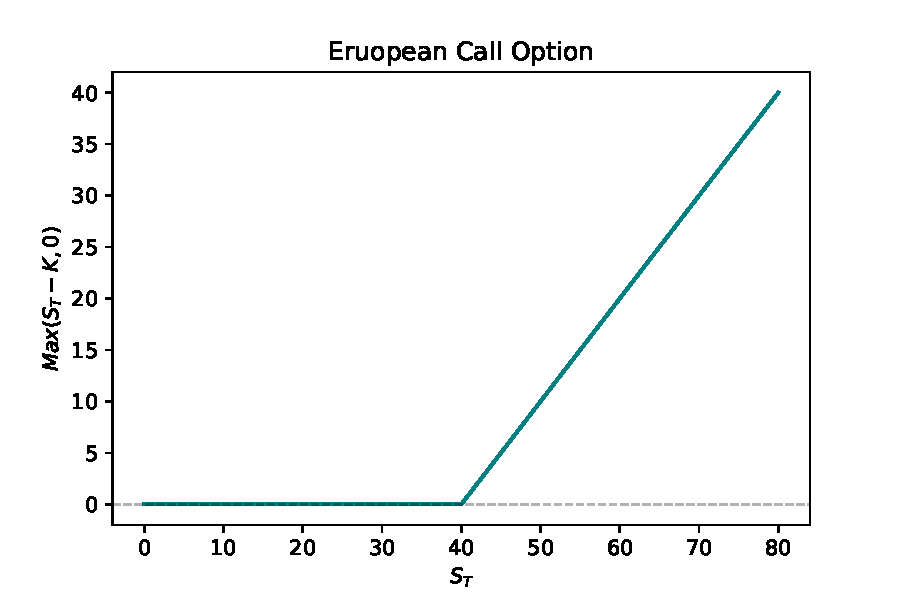
\includegraphics[width=0.7\textwidth]{../images/Call.pdf}	
	\caption{European Call Payoff}
\end{figure}

Note that the payoff of this derivative is \textit{stochastic} in sense that we cannot be certain of the price the stock will reach some future time from now. Then, we cannot be sure of the future payoff of the stock.\\

The knowledge and tools we currently have can take us only so far if we desire to compute the proper price for an option, such that hedges the position of the seller. Under this constraint, we require to properly take account of the randomness of the stock, in pursuance of the \textit{right} way to price this derivative.

\end{document}